\chapter{Example Content}
This section showcases the way I formatted my lists, tables, equations, etc. If you decide to do it differently, then you'll be on your own to debug any subsequent formatting problems.

The structure of this chapter is as follows: \secref{sec:mySection} showcases the use of SSSSR sections. \secref{sec:LineBreaks} discusses the use of line breaks in section headings. \secref{sec:ContentTypes} shows how to display many different types of content.


%%%%%%%%%%%%%%%%%%%%%%%%%%%%%%%%%%%%%%%%%%%%%%%%%%%%%%%%%%%%%%%%%%%%%%%%%%%%%%%%%
%%%%%%%%%%%%%%%%%%%%%%%%%%%%%%%%%%%%%%%%%%%%%%%%%%%%%%%%%%%%%%%%%%%%%%%%%%%%%%%%%
\section{Displaying Sections} \label{sec:mySection}
This section has many subsections, which I can refer to by their labels. e.g. \secref{sec:mySection}, \secref{ssec:mySubsection}, \secref{sssec:ShinySmilyStory}, \secref{ssssec:SSSSGridman}, \secref{sssssec:Snake}, and \secref{ssec:SuperSuperRareBotan}.

Labeling sections is optional. Labels may be anything, but must be unique (hence my naming convention).

Example text.


%%%%%%%%%%%%%%%%%%%%%%%%%%%%%%%%%%%%%%%%%%%%%%%%%%%%%%%%%%%%%%%%%%%%%%%%%%%%%%%%%
\subsection{My Subsection} \label{ssec:mySubsection}
Example text.


%%%%%%%%%%%%%%%%%%%%%%%%%%%%%%%%%%%%%%%%%%%%%%%%%%%%%%%%%%%%%%%%%%%%%%%%%%%%%%%%%
\subsubsection{My Subsubsection} \label{sssec:ShinySmilyStory}
Example text.


%%%%%%%%%%%%%%%%%%%%%%%%%%%%%%%%%%%%%%%%%%%%%%%%%%%%%%%%%%%%%%%%%%%%%%%%%%%%%%%%%
\paragraph{My Subsubsubsection... WAIT WHAT!?} \label{ssssec:SSSSGridman}
If you get this deep, the command is not `subsubsubsection', but `paragraph'. Why?

For the record, I suggest not to use this much depth unless you've really thought about your structure, and you are sure that it is the best way to do it.


%%%%%%%%%%%%%%%%%%%%%%%%%%%%%%%%%%%%%%%%%%%%%%%%%%%%%%%%%%%%%%%%%%%%%%%%%%%%%%%%%
\subparagraph{My Subsubsubsubsection... rofl} \label{sssssec:Snake}
This is the maximum section depth that the titlesec package defines. May you never need it.


%%%%%%%%%%%%%%%%%%%%%%%%%%%%%%%%%%%%%%%%%%%%%%%%%%%%%%%%%%%%%%%%%%%%%%%%%%%%%%%%%
\subsection{My Other Subsection} \label{ssec:SuperSuperRareBotan}
Example text.


%%%%%%%%%%%%%%%%%%%%%%%%%%%%%%%%%%%%%%%%%%%%%%%%%%%%%%%%%%%%%%%%%%%%%%%%%%%%%%%%%
%%%%%%%%%%%%%%%%%%%%%%%%%%%%%%%%%%%%%%%%%%%%%%%%%%%%%%%%%%%%%%%%%%%%%%%%%%%%%%%%%
\section[Displaying Different Text In The Contents]{Displaying Different Text\\In The Contents\\Because You Can}  \label{sec:LineBreaks}
The heading in this section is different to the heading in the table of contents. You can use this method if you wish to force line breaks in your heading, but not in the contents.


%%%%%%%%%%%%%%%%%%%%%%%%%%%%%%%%%%%%%%%%%%%%%%%%%%%%%%%%%%%%%%%%%%%%%%%%%%%%%%%%%
%%%%%%%%%%%%%%%%%%%%%%%%%%%%%%%%%%%%%%%%%%%%%%%%%%%%%%%%%%%%%%%%%%%%%%%%%%%%%%%%%
\section{Displaying Different Types of Content} \label{sec:ContentTypes}


%%%%%%%%%%%%%%%%%%%%%%%%%%%%%%%%%%%%%%%%%%%%%%%%%%%%%%%%%%%%%%%%%%%%%%%%%%%%%%%%%
\subsection{Citations}
This is a citation \cite{example1}, and this is another \cite{example1,example2,example4,example5}.

This is a footnote\footnote{Source: \href{https://www.example.com/}{Example}.}. The text continues.


%%%%%%%%%%%%%%%%%%%%%%%%%%%%%%%%%%%%%%%%%%%%%%%%%%%%%%%%%%%%%%%%%%%%%%%%%%%%%%%%%
\subsection{Lists}
An example list is as follows:
\begin{enumerate}[topsep=0pt,beginpenalty=10000,first=\interlinepenalty10000]
    \item This is a list
    \item This is a list
    \item This is a list
\end{enumerate}


%%%%%%%%%%%%%%%%%%%%%%%%%%%%%%%%%%%%%%%%%%%%%%%%%%%%%%%%%%%%%%%%%%%%%%%%%%%%%%%%%
\subsection{Quotes}
Quotes can be used as follows

Inline quotes can use `single' or ``double'' quotes like this. To this, Brandon stated:

\vspace*{-\parskip}
\begin{displayquote}
	``Turtles are cute.''
\end{displayquote}


%%%%%%%%%%%%%%%%%%%%%%%%%%%%%%%%%%%%%%%%%%%%%%%%%%%%%%%%%%%%%%%%%%%%%%%%%%%%%%%%%
\subsection{Figures}
This is a figure reference: \figref{fig:Example1}

Some different ways to show figures include full page width (\figref{fig:Example1}), side-by-side (\figref{fig:Example2} and \figref{fig:Example3}), and subfigures (\figref{fig:Example4} which consists of \figref{fig:Example4a} and \figref{fig:Example4b}).

If you have mathematical symbols in your figures and you're using inkscape, you can input latex maths into the figure with: Extensions > Render > Formula (pdflatex).

\begin{figure}[!htb]
	\centering
	\centerline{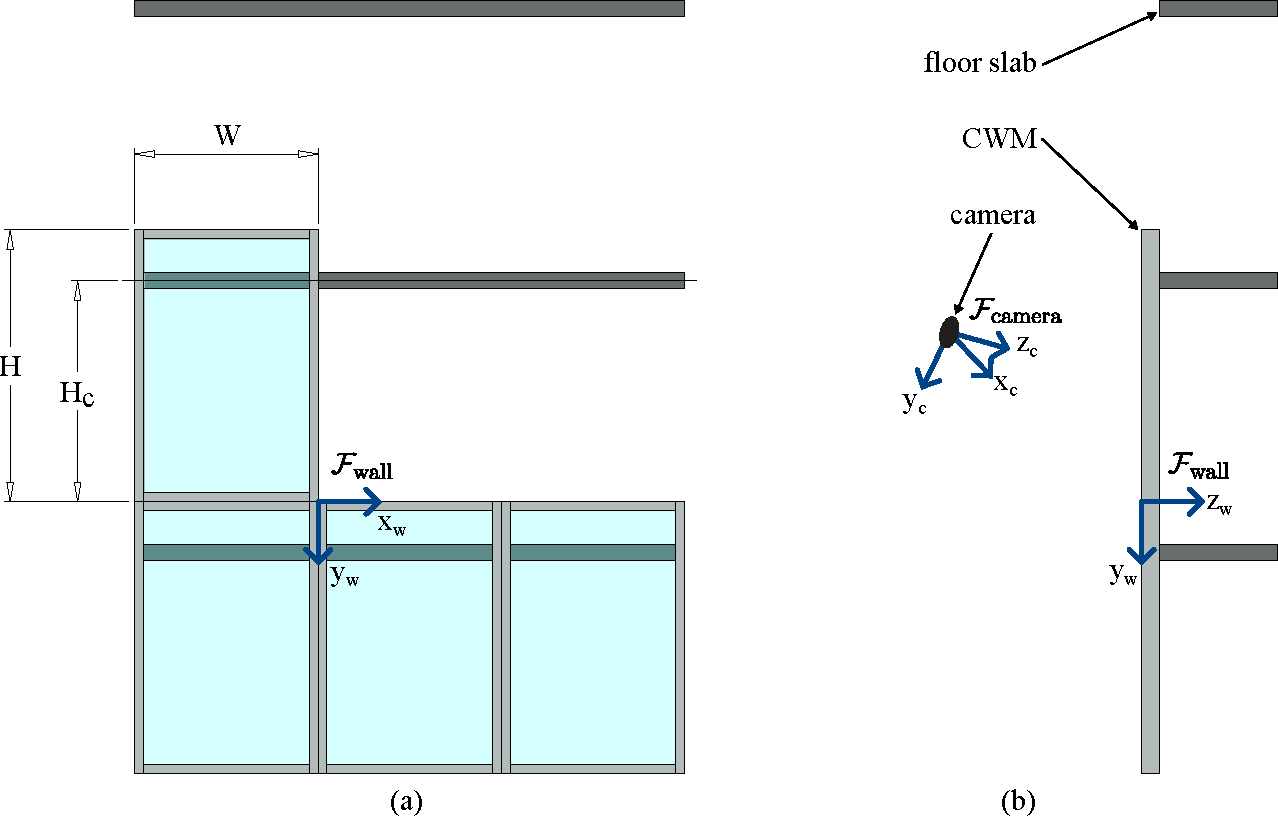
\includegraphics[width=\textwidth,keepaspectratio]{Figures/ExampleFigure3.pdf}}
	\caption{Export your graphics to pdf. Lovely vector graphics! If I see any jpeg text I am sad.}
	\label{fig:Example1}
\end{figure}

\begin{figure}[!htb]
	\centering
	\captionbox{Cool graphic!\label{fig:Example2}}
		[.5\textwidth]{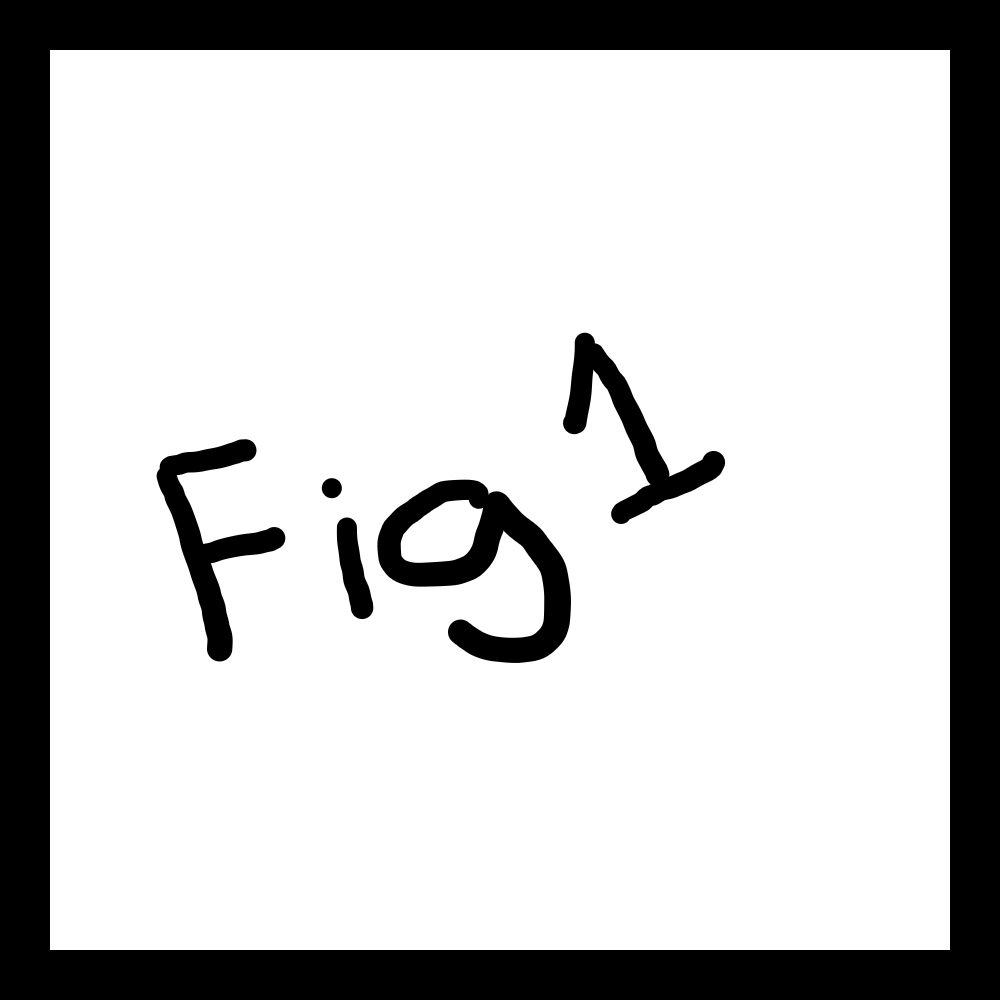
\includegraphics[width=0.5\textwidth,keepaspectratio]{Figures/ExampleFigure1.png}}%%
	\captionbox{This is a very long caption that takes up multiple lines.\label{fig:Example3}}
		[.5\textwidth]{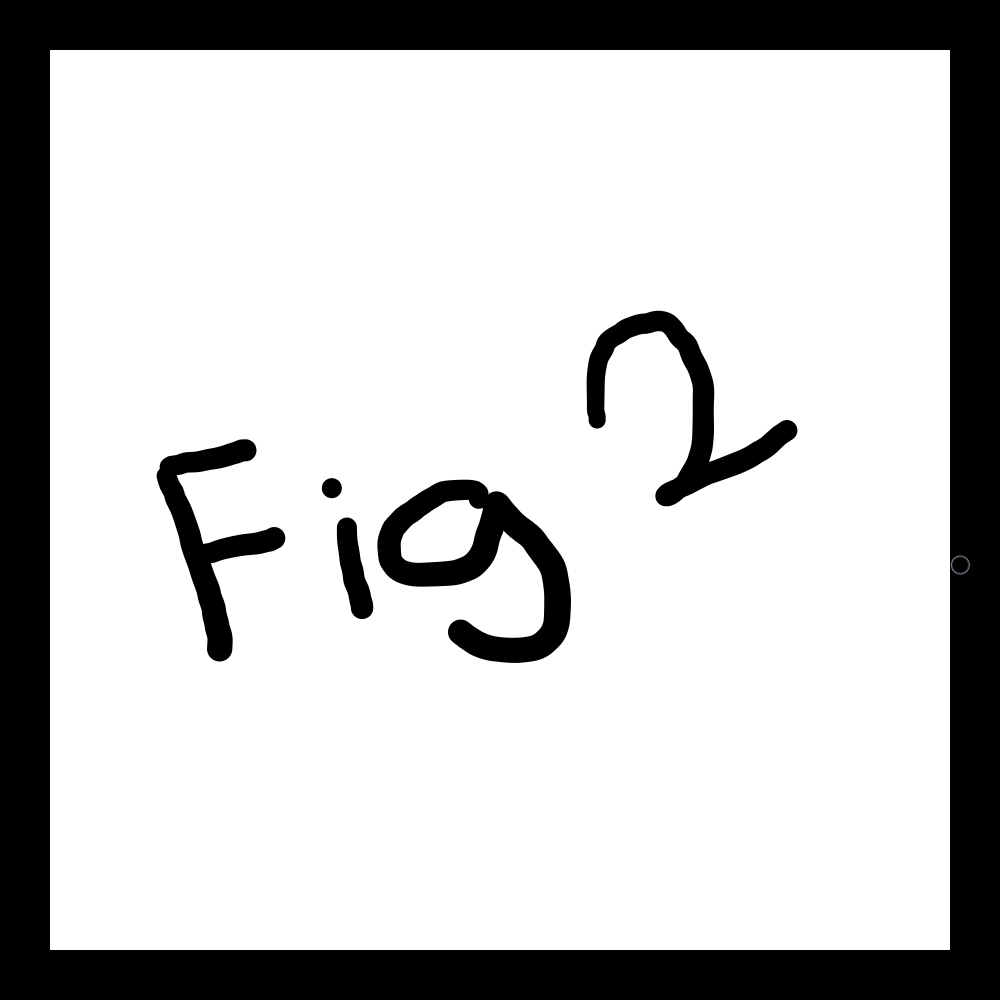
\includegraphics[width=0.5\textwidth,keepaspectratio]{Figures/ExampleFigure2.png}}
\end{figure}

\begin{figure}[!htb]
	\centering
    \begin{subfigure}[t]{0.49\textwidth}
        \centering
		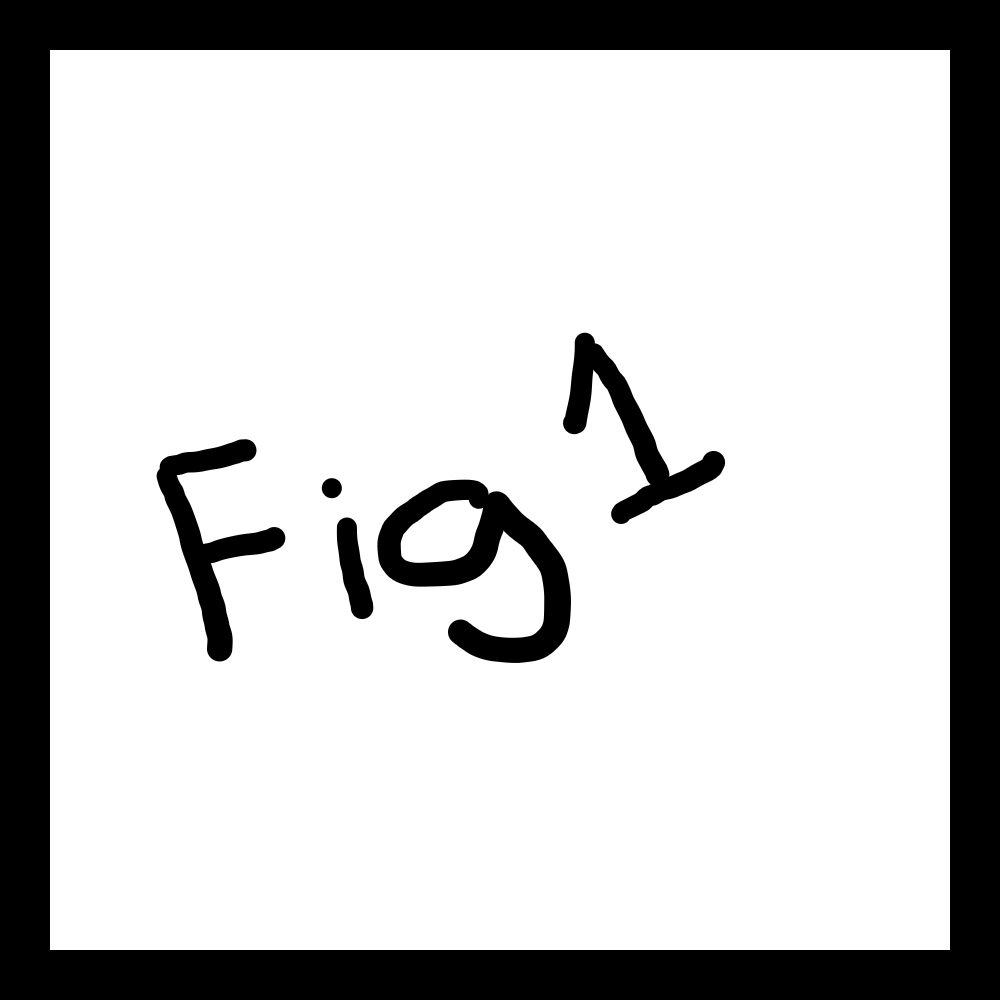
\includegraphics[width=\textwidth,keepaspectratio]{Figures/ExampleFigure1.png}
	    \caption{Cool graphic!}
        \label{fig:Example4a}
    \end{subfigure}
    \begin{subfigure}[t]{0.49\textwidth}
        \centering
		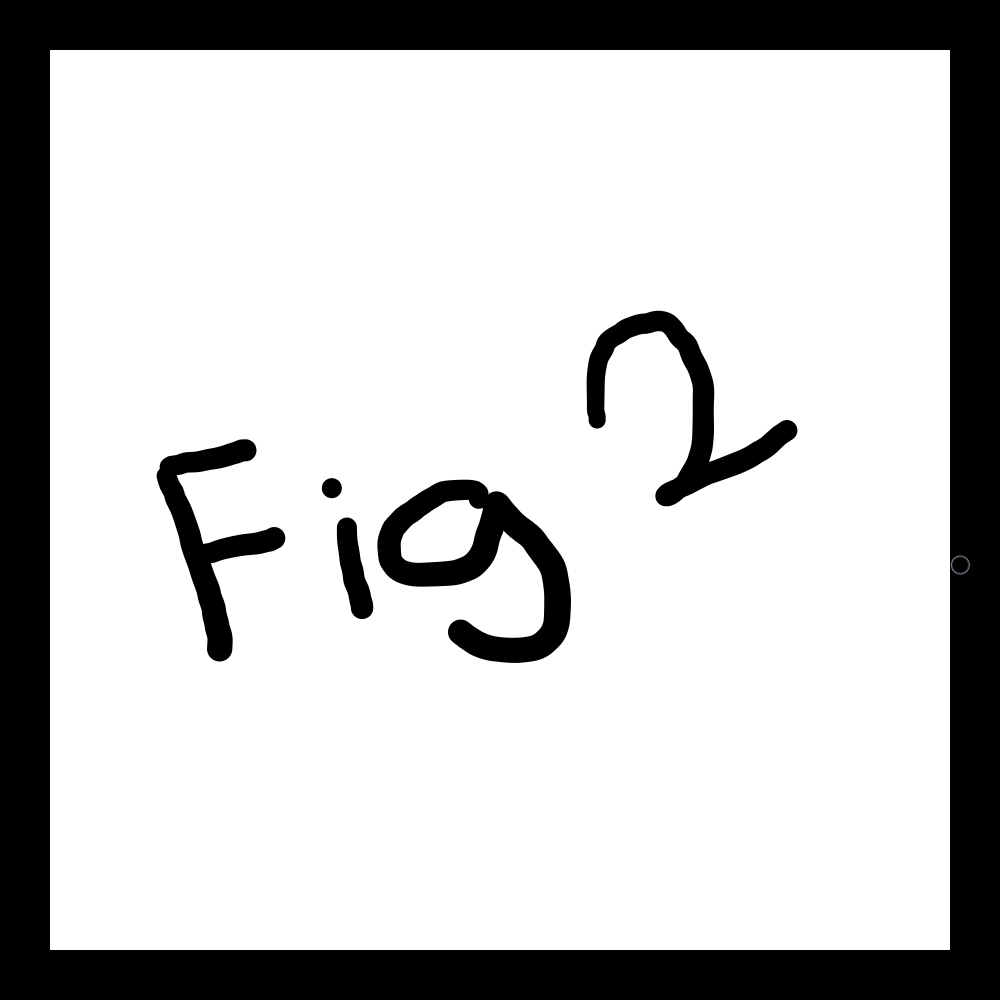
\includegraphics[width=\textwidth,keepaspectratio]{Figures/ExampleFigure2.png}
	    \caption{This is a very long caption that takes up multiple lines.}
        \label{fig:Example4b}
    \end{subfigure}
    \caption{Cool graphics!}
    \label{fig:Example4}
\end{figure}


%%%%%%%%%%%%%%%%%%%%%%%%%%%%%%%%%%%%%%%%%%%%%%%%%%%%%%%%%%%%%%%%%%%%%%%%%%%%%%%%%
\subsection{Equations}
This is an equation reference: \eqref{eq:myEq}.

\begin{equation} \label{eq:myEq}
    a = 2
\end{equation}

where $a$ is a variable.


%%%%%%%%%%%%%%%%%%%%%%%%%%%%%%%%%%%%%%%%%%%%%%%%%%%%%%%%%%%%%%%%%%%%%%%%%%%%%%%%%
\subsection{Tables}

This is a table reference: \tbref{tb:myTable}.

This is a fairly basic table. See threeparttable if you want table notes (footnotes for tables). For more fancy tables, use NiceTabular of the package NiceMatrix.

\begin{table}[!h]
    \centering
    \begin{tabular}{llll}
        \hline
        & & \multicolumn{2}{l}{Measurement error}\\
        Measurement & Unit & Mean & Standard deviation\\
        \hline
        $x_n$ & mm & 5.2 & 8.6\\
        $y_n$ & mm & 3.5 & 3.0\\
        $z_n$ & mm & -6.5 & 9.1\\
        $\theta_q$ & degrees & 1.6$\degree$ & 2.9$\degree$\\
        \hline
        \end{tabular}
    \caption{Average measurement error over all 99 successful measurements. $(x_n, y_n, z_n)$ are defined somewhere else. $\theta_q$ is the rotational misalignment as a quaternion angular distance.}
    \label{tb:myTable}
\end{table}


%%%%%%%%%%%%%%%%%%%%%%%%%%%%%%%%%%%%%%%%%%%%%%%%%%%%%%%%%%%%%%%%%%%%%%%%%%%%%%%%%
\subsection{Algorithms}

\begin{algorithm}
    \DontPrintSemicolon
    %% SYNTAX: \SetKwProg{CommandName}{Title}{ is}{end}
    \SetKwProg{Fn}{Function}{}{end}
    %% SYNTAX: \Set...{CommandName}{TextToDisplay}
    \SetKwFunction{Multiply}{Multiply}
    \SetKwInOut{TypeDefLength}{Length}
    \SetKwInOut{TypeDefArea}{Area}
    \SetKwIF{If}{ElseIf}{Else}{if}{}{else if}{else}{end} %% Actual IF statement (remove the "then")
    \SetKwIF{InputBlock}{}{}{Input}{}{}{}{end}{} %% Not an IF statement, just using the block structure
    \SetKwInOut{InputDefL}{$L$}
    \SetKwInOut{InputDefW}{$W$}
    %% START PRINTING
    \emph{Type Definitions}\\
    \TypeDefLength{A length measurement, with units in mm}
    \TypeDefArea{An area measurement, with units in $\text{mm}^\text{2}$}
    \BlankLine
    \nl \Fn{\Multiply}{
        %\ResetInOut{xx} %% This macro sets a fixed distance based on the text INSIDE IT..... WHY?
        \InputBlock{}{
            \InputDefL{[\KwSty{Length}] Object length}
            \InputDefW{[\KwSty{Length}] Object width}
        }
        \BlankLine
        \lnl{algo:M:vStart} \uIf{$L < 0$}{
            \lnl{algo:M:errorL} \KwRet{Bad input: L}
        }
        \nl \uElseIf{$W < 0$}{
            \lnl{algo:M:errorW} \KwRet{Bad input: W}
        }
        \nl \Else{
            \lnl{algo:M:vEnd} Carry on citizen\;
        }
        \lnl{algo:M:start} Copy $L$ into the calculator\;
        \lnl{algo:M:t} press the $\times$ button on the calculator\;
        \lnl{algo:M:w} Copy $W$ into the calculator\;
        \lnl{algo:M:e} Press the $=$ button on the calculator\;
        \lnl{algo:M:r} \KwSty{Area} $A \leftarrow$ The result shown on the calculator\;
        \BlankLine
        \lnl{algo:M:return} \KwRet{$A$, The area as measured in units of {\normalfont $\text{mm}^\text{2}$}}
    }
    \caption{Algorithm to find the area of an object.}
    \label{alg:myAlgo}
\end{algorithm}

Pseudocode of the  algorithm is \algoref{alg:myAlgo}. In the first stage of the algorithm, \algoRefLines{algo:M:vStart}{algo:M:vEnd} validate the inputs. Then \algoRefLines{algo:M:start}{algo:M:r} do the calculation. Then \algoRefLine{algo:M:return} outputs the result.
